% !TEX program = xelatex
\documentclass[10pt,letterpaper,twocolumn]{article}

% === PAGE ===
\usepackage[top=0.75in,bottom=0.75in,left=0.75in,right=0.75in,footskip=12pt]{geometry}

% === FONTS ===
\usepackage{fontspec}
\usepackage{unicode-math}
\setmainfont{Latin Modern Roman}[
  Extension=.otf,
  UprightFont=lmroman10-regular,
  BoldFont=lmroman10-bold,
  ItalicFont=lmroman10-italic,
  BoldItalicFont=lmroman10-bolditalic,
]
\setsansfont{Latin Modern Sans}[
  Extension=.otf,
  UprightFont=lmsans10-regular,
  BoldFont=lmsans10-bold,
  ItalicFont=lmsans10-oblique,
  BoldItalicFont=lmsans10-boldoblique,
]
\setmonofont{Latin Modern Mono}[
  Extension=.otf,
  UprightFont=lmmono10-regular,
  ItalicFont=lmmono10-italic,
  Scale=0.85,
]
\newfontfamily\acbold{ywft-processing-bold}[
  Path=../../system/public/type/webfonts/,
  Extension=.ttf
]

% === PACKAGES ===
\usepackage{xcolor}
\usepackage{titlesec}
\usepackage{enumitem}
\usepackage{booktabs}
\usepackage{tabularx}
\newcolumntype{Y}{>{\RaggedRight\arraybackslash}X}
\usepackage{fancyhdr}
\usepackage{hyperref}
\usepackage{xurl}
\usepackage{graphicx}
\graphicspath{{./}{figures/}}
\usepackage{ragged2e}
\usepackage{microtype}
\usepackage[font=footnotesize]{caption}
\usepackage{natbib}
\usepackage{tikz}
\usetikzlibrary{arrows.meta,calc,positioning}
\usepackage{../ac-source-bundle}

% === COLORS ===
\definecolor{acpink}{RGB}{180,72,135}
\definecolor{acpurple}{RGB}{120,80,180}
\definecolor{acdark}{RGB}{64,56,74}
\definecolor{acgray}{RGB}{119,119,119}
\definecolor{acblue}{RGB}{42,100,212}

\hypersetup{
  colorlinks=true,
  linkcolor=acpurple,
  urlcolor=acpurple,
  citecolor=acpurple,
  pdfauthor={@jeffrey},
  pdftitle={Free Versus Nonfree: Stallman's Licensing Map and Where Aesthetic.Computer Stands},
}

% === SECTIONS ===
\titleformat{\section}{\normalfont\bfseries\normalsize\uppercase}{\thesection.}{0.5em}{}
\titlespacing{\section}{0pt}{1.2em}{0.3em}
\titleformat{\subsection}{\normalfont\bfseries\small}{\thesubsection}{0.5em}{}
\titlespacing{\subsection}{0pt}{0.8em}{0.2em}

% === RUNNING MATTER ===
\pagestyle{fancy}
\fancyhf{}
\renewcommand{\headrulewidth}{0pt}
\fancyfoot[C]{\footnotesize\thepage}
\setlist[itemize]{nosep,leftmargin=1.2em,itemsep=0.1em}
\setlist[enumerate]{nosep,leftmargin=1.2em}
\setlength{\columnsep}{1.8em}
\setlength{\parindent}{1em}
\setlength{\parskip}{0.3em}
\tolerance=800
\emergencystretch=1em
\hyphenpenalty=50

\newcommand{\acdot}{{\color{acpink}.}}
\newcommand{\ac}{Aesthetic{\acdot}Computer}
\newcommand{\code}[1]{\texttt{#1}}
\newcommand{\term}[1]{``#1''}
\newcommand{\coverplate}{%
  \begin{tikzpicture}
    \node[inner sep=0pt,outer sep=0pt,rounded corners=14pt,fill=acpink!6]
      {
\includegraphics[width=0.40\textwidth]{figures/cover}};
  \end{tikzpicture}%
}

\InputIfFileExists{version}{}{%
  \providecommand{\paperhash}{dev}\providecommand{\paperrev}{?}}

\newcommand{\plang}[2]{\href{https://papers.aesthetic.computer/free-vs-open-26-arxiv#2.pdf}{\color{acgray}#1}}
\newcommand{\planghere}[1]{{\bfseries\color{acpink}#1}}
\newcommand{\plangsep}{{\color{acgray!60}\,\textperiodcentered\,}}

\begin{document}

\twocolumn[{%
\begin{center}
{\acbold\fontsize{26pt}{30pt}\selectfont\color{acdark} Free Versus Nonfree}\par
\vspace{0.45em}
{\itshape\fontsize{14pt}{17pt}\selectfont\color{acpink} Stallman's Licensing Map, the 1998 Split, and Where \ac{} Stands}\par
\vspace{0.5em}
\coverplate\par
\vspace{0.5em}
{\small\color{acgray} \href{https://prompt.ac/@jeffrey}{@jeffrey} \,\textperiodcentered\, \ac{} \,\textperiodcentered\, ORCID \href{https://orcid.org/0009-0007-4460-4913}{0009-0007-4460-4913} \,\textperiodcentered\, September 2026}\par
\vspace{0.45em}
{\footnotesize\sffamily\planghere{EN}\plangsep\plang{DA}{-da}\plangsep\plang{ES}{-es}\plangsep\plang{ZH}{-zh}\plangsep\plang{JA}{-ja}}\par
\vspace{0.55em}
{\color{acpink}\rule{\textwidth}{1.2pt}}
\vspace{0.5em}
\end{center}

\begin{quote}
\small\noindent\textbf{Abstract.}
Software licensing is usually explained as a spectrum from \term{open} to \term{closed.} Richard Stallman rejects that axis, and his rejection is the subject of this paper. Reading his two essays on the question, the 1998 original \emph{Why ``Free Software'' is better than ``Open Source''} and its 2007 rewrite \emph{Why Open Source Misses the Point of Free Software}, alongside the GNU Project's category and vocabulary pages, I reconstruct his map: one ethical line between \emph{free} and \emph{nonfree}, drawn by four user freedoms, with a second line inside the free region between \emph{copyleft} and \emph{lax} licensing, and commerce as an orthogonal axis. I trace what changed between the two essays, including the later attention to tivoization, trademark conditions, and the \term{source-available} misreading. The paper then applies the map to \ac{} itself. The monorepo is public and its manifests declare the ISC license, a lax license, but no license text is tracked in the tree. On Stallman's map this makes the project source-available rather than clearly free. I close with what a deliberate placement would require and why the choice matters for a platform whose users publish works into it.
\end{quote}
\vspace{0.5em}
}]

\section{The Question Is the Vocabulary}

A friend asked me about \term{Stallman's licensing regimes, open versus closed source.} The phrasing contains the thing Stallman most objects to. In both of his essays on the subject he writes that what the free software movement advocates \term{is not `open source,' and what we oppose is not `closed source'}~\citep{stallman2007misses}. The words are the argument. This paper explains the map he draws instead, records how it changed between 1998 and 2007, and then does the exercise he would ask of any project: it locates \ac{} on that map using the repository as evidence.

The paper is expository rather than adversarial. Stallman's claims are stated as his, in his terms, with page sources. Where the platform's own record contradicts his ideal, the record is reported and not smoothed.

\section{Sources and Method}

The Platter consulted for this paper is small and public. The primary texts are two essays on gnu.org and three reference pages: the free software definition, the category page, and the \emph{Words to Avoid} list~\citep{stallman1998better,stallman2007misses,gnu_freesw,stallman_categories,gnu_words}. The 1998 essay carries a header stating it \term{has been superseded by a major rewrite} and is \term{kept for historical reasons}; its copyright line runs 1998--2003, 2007, 2010, 2023, 2024. The 2007 rewrite's copyright line runs 2007 through 2024, so it is still being revised. Both were fetched on September 15, 2026, and their plain-text extractions sit in the source bundle attached at the end of this PDF.

Stallman's personal site, \code{stallman.org}, was also checked, since the original request assumed the essay lived there. Its article index holds political and personal writing and points readers to \code{gnu.org/philosophy} for everything about software. Nothing on the licensing question is hosted there.

Prior \ac{} papers that touch the subject are \emph{Get Closed Source Out of Schools}, which cites Stallman for the claim that users deserve control over the software they run, and \emph{Pieces Not Programs} and \emph{Keymaps as Social Software}, which define the unit of authorship and the versioned object that any license here would have to cover~\citep{scudder2026openschools,scudder2026pieces,scudder2026keymaps}. For the platform's own license state I inspected the checked-out monorepo on September 15, 2026~\citep{acrepo2026}.

\section{The Four Freedoms}

\begin{figure*}[t]
\centering
\resizebox{0.96\textwidth}{!}{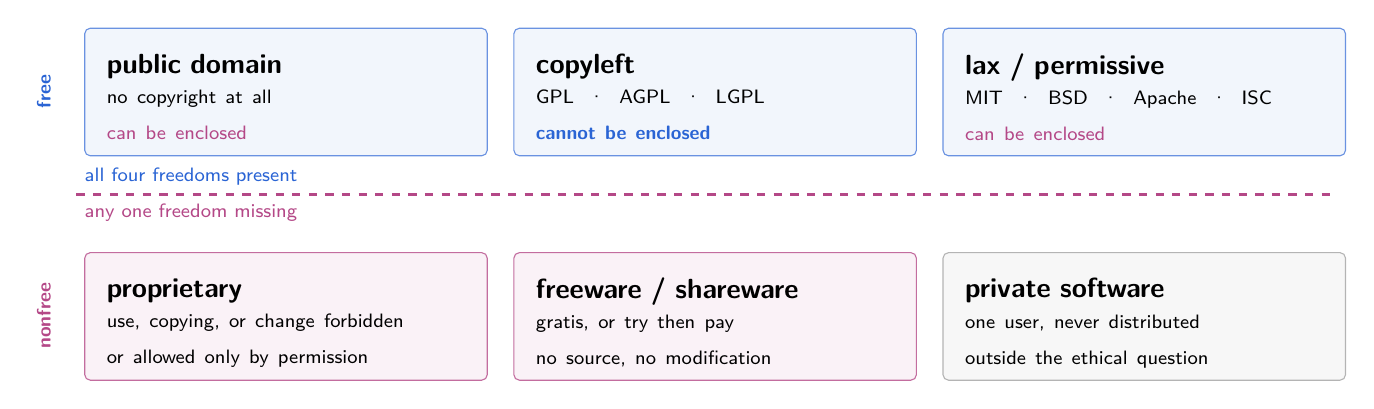
\begin{tikzpicture}[
  every node/.style={font=\sffamily},
  tier/.style={draw=acgray!55, rounded corners=2pt, fill=white, align=left, anchor=north west,
    minimum height=1.62cm, text width=4.55cm, inner xsep=8pt, inner ysep=6pt, text depth=0.72cm},
  free/.style={tier, draw=acblue!70, fill=acblue!6},
  nonfree/.style={tier, draw=acpink!80, fill=acpink!7},
  aside/.style={tier, draw=acgray!55, fill=acgray!6},
  side/.style={font=\scriptsize\sffamily\bfseries, anchor=east},
  lab/.style={font=\scriptsize\sffamily, text=acpink, anchor=west, inner xsep=0pt}
]
  \def\colA{0}\def\colB{5.45}\def\colC{10.9}
  \def\rowA{0}\def\rowB{-2.85}

  % free row
  \node[free] at (\colA,\rowA) {\textbf{public domain}\\[-1pt]{\scriptsize no copyright at all}\\[1pt]{\scriptsize\color{acpink} can be enclosed}};
  \node[free] at (\colB,\rowA) {\textbf{copyleft}\\[-1pt]{\scriptsize GPL \;\textperiodcentered\; AGPL \;\textperiodcentered\; LGPL}\\[1pt]{\scriptsize\color{acblue}\bfseries cannot be enclosed}};
  \node[free] at (\colC,\rowA) {\textbf{lax / permissive}\\[-1pt]{\scriptsize MIT \;\textperiodcentered\; BSD \;\textperiodcentered\; Apache \;\textperiodcentered\; ISC}\\[1pt]{\scriptsize\color{acpink} can be enclosed}};

  % the line
  \draw[dashed, draw=acpink, line width=0.9pt] (-0.1,-2.12) -- (15.85,-2.12);
  \node[lab, text=acblue] at (0,-1.89) {all four freedoms present};
  \node[lab] at (0,-2.35) {any one freedom missing};

  % nonfree row
  \node[nonfree] at (\colA,\rowB) {\textbf{proprietary}\\[-1pt]{\scriptsize use, copying, or change forbidden}\\[1pt]{\scriptsize or allowed only by permission}};
  \node[nonfree] at (\colB,\rowB) {\textbf{freeware / shareware}\\[-1pt]{\scriptsize gratis, or try then pay}\\[1pt]{\scriptsize no source, no modification}};
  \node[aside] at (\colC,\rowB) {\textbf{private software}\\[-1pt]{\scriptsize one user, never distributed}\\[1pt]{\scriptsize outside the ethical question}};

  % side labels
  \node[side, text=acblue] at (-0.3,-0.81) {\rotatebox{90}{free}};
  \node[side, text=acpink] at (-0.3,-3.66) {\rotatebox{90}{nonfree}};
\end{tikzpicture}
}
\caption{Stallman's categories, arranged around the one line he treats as ethical. Public domain and lax-licensed code are free but can be enclosed into a proprietary product. Copyleft code cannot: every redistributed copy must carry the same freedoms. Private software, written for one user and never distributed, sits outside the question because nobody else's freedom is at stake~\citep{stallman_categories}.}
\label{fig:ladder}
\end{figure*}

Stallman's definition of free software has been stable since 1986 and is the test everything else in his map depends on. A program is free software if its users have four freedoms (Table~\ref{tab:freedoms}). Freedom is a property of the user's relation to the program, not of the program's price and not of the visibility of its source. Missing any one freedom makes the program \emph{nonfree}, which he also calls \emph{proprietary}.

\begin{table}[t]
\small
\centering
\begin{tabularx}{\columnwidth}{@{}l Y@{}}
\toprule
\textbf{Freedom} & \textbf{What the user may do} \\
\midrule
0 & Run the program as you wish, for any purpose. \\
1 & Study how the program works, and change it so it does your computing as you wish. Access to the source code is a precondition. \\
2 & Redistribute copies so you can help others. \\
3 & Distribute copies of your modified versions to others. Access to the source code is a precondition. \\
\bottomrule
\end{tabularx}
\caption{The four freedoms, numbered from zero as the GNU definition numbers them. A program is free software only if its users have all four~\citep{gnu_freesw}.}
\label{tab:freedoms}
\end{table}

The definition contains the response to the phrase \term{free as in beer.} Both essays repeat the line: think of \term{free speech,} not \term{free beer.} Stallman concedes in both that the English word is ambiguous and that every proposed replacement, including \term{open source,} has \term{some kind of semantic problem.} His claim is that \term{free software} has two natural readings, one of which is correct, so a reader who has once been corrected does not go wrong again, while \term{open source} has one natural reading, \term{you can look at the source code,} and that reading is wrong~\citep{stallman2007misses}.

\section{The Map}

With the four freedoms as the test, Stallman's category page sorts software into tiers~\citep{stallman_categories}. Figure~\ref{fig:ladder} draws them. The only hard line is between free and nonfree. Above the line, the tiers differ in how well freedom survives redistribution. Below it, they differ in price and in how much the owner permits.

\subsection{Above the line}

\textbf{Public domain} software has no copyright. It is free, but noncopyleft: anyone may take it, add restrictions, and distribute the result as proprietary software.

\textbf{Copyleft} software is licensed so that every copy, modified or not, must be redistributed under the same terms. The GNU General Public License is the canonical instrument. The AGPL extends the obligation to software run as a network service, closing the gap through which a modified server program is used by the public but never \term{distributed.} The LGPL is a deliberately weaker copyleft that lets proprietary programs link to a library without inheriting the license. Stallman's own account of why he chose copyleft is titled \emph{Copyleft: Pragmatic Idealism}: the goal is freedom, and copyleft is the mechanism that keeps it from leaking~\citep{stallman_pragmatic}.

\textbf{Lax} or \textbf{permissive} software is free but noncopyleft: MIT, the BSD family, Apache, ISC. The category page calls these \term{lax, permissive} licenses and notes they allow the code to be made proprietary. In more pointed passages he has called them \term{pushover} licenses. This tier is where most contemporary JavaScript lives, and it is where \ac{}'s manifests place the project.

\subsection{Below the line}

\textbf{Proprietary} software forbids use, copying, or modification, or requires permission for them. For Stallman this is an injustice to the user regardless of price. \textbf{Freeware} is gratis and redistributable but ships no source and forbids modification; he asks that the word not be used for free software. \textbf{Shareware} may be passed around but continued use requires a fee. \textbf{Private software}, written for one user and never distributed, is the one tier below the line that raises no ethical problem: if that one user holds the four freedoms, nobody else is affected, and most custom in-house software is this.

\subsection{Commerce is a different axis}

Stallman insists that \emph{commercial} is orthogonal to \emph{free}. Commercial means developed or sold as a business activity. Free software can be commercial, and he encourages it; nonfree software can be gratis (Table~\ref{tab:axes}). The conflation is what lets \term{free} get heard as \term{unpaid,} so the category page treats it as an error worth its own entry.

\begin{table}[t]
\small
\centering
\begin{tabularx}{\columnwidth}{@{}l Y Y@{}}
\toprule
 & \textbf{noncommercial} & \textbf{commercial} \\
\midrule
\textbf{free} & hobby GPL projects; most of a distribution's long tail & paid GPL support and enterprise distributions; legitimate and encouraged \\
\addlinespace
\textbf{nonfree} & freeware; \term{free for personal use} downloads & ordinary proprietary software; most of the industry \\
\bottomrule
\end{tabularx}
\caption{Freedom and commerce as independent axes. Stallman's objection is to the bottom row, not the right column~\citep{stallman_categories}.}
\label{tab:axes}
\end{table}

\section{1998 and 2007: What Changed}

The two essays make the same argument, but the later one is longer, calmer, and more specific about how \term{open source} fails in practice. Table~\ref{tab:essays} aligns their sections.

\begin{table*}[t]
\small
\centering
\begin{tabularx}{\textwidth}{@{}Y Y Y@{}}
\toprule
\textbf{1998 original} & \textbf{2007 rewrite} & \textbf{What the rewrite adds} \\
\midrule
Relationship between the two movements & (folded into the opening) & The open source idea \term{values mainly practical advantage and does not campaign for principles.} \\
Comparing the two terms; Ambiguity & Common Misunderstandings of the two terms & The \term{source available} term for the naive reading; \term{open source} stretched to government, education, and science until it means only \term{participatory.} \\
--- & Practical Differences & Open Watcom's license, trademark conditions on the Rust compiler, and \emph{tivoization}: free source compiled into a signed executable the user cannot replace. \\
--- & Different Values Can Lead to Similar Conclusions---but Not Always & The two camps react differently to a good proprietary program: the enthusiast asks for a copy, the activist declines and funds a replacement. \\
--- & Powerful, Reliable Software Can Be Bad & DRM and \term{open source DRM}: power and reliability serve the user only if the software respects the user. \\
Fear of Freedom & Fear of Freedom & Same section, expanded; the \term{gift to humanity} framing presumes proprietary release is legitimate. \\
Would a Trademark Help?; Misunderstandings(?) of \term{Open Source} & --- & The IBM and Cygnus announcements are dropped; the trademark argument is dropped. \\
--- & \term{FLOSS} and \term{FOSS} & FLOSS is the neutral term if neutrality is the goal; neutrality is not the goal. \\
--- & Rivals for Mindshare & \term{Free} and \term{open} compete for the same conceptual slot; decline to work on activities that call themselves \term{open.} \\
\bottomrule
\end{tabularx}
\caption{Section alignment of the 1998 essay and the 2007 rewrite, from the fetched texts of September 15, 2026~\citep{stallman1998better,stallman2007misses}. Both share the closing line: say \term{it's free software and it gives you freedom!} more and louder than before.}
\label{tab:essays}
\end{table*}

\subsection{The split}

Both essays date the split to 1998, when \term{a part of the free software community splintered off and began campaigning in the name of `open source'\,} The Open Source Initiative's own history records the February 3, 1998 meeting in Palo Alto at which the term was adopted, and its definition is a lightly edited copy of the Debian Free Software Guidelines~\citep{osi_history,osi_definition}. Stallman does not dispute that the licenses overlap almost entirely. His claim is about what the rebrand was for. The 1998 essay quotes the line that has become the standard summary, attributed only to \term{one person}: \term{open source is a development methodology; free software is a social movement.} The 2007 rewrite drops the quotation and states the difference in his own voice: for open source, nonfree software is \term{an inferior solution to the practical problem at hand}; for free software it is \term{a social problem, and the solution is to stop using it.}

\subsection{Not enemies}

A point that is easy to miss when the essays are read as polemic: both insist that the open source camp is not the enemy. \term{The enemy is proprietary software.} The 1998 version spends a section rejecting the comparison to factional radical groups of the 1960s, and the 2007 version keeps it, adding that the two camps \term{often work together on practical projects.} What he refuses is being \emph{lumped in}: the free software movement built the community and does not accept being credited to a philosophy that omits its reason for existing.

\subsection{What practice taught him}

The 2007 rewrite's genuinely new material is the section on practical differences, and it reads as a list of cases the intervening decade produced. The first is a license (Open Watcom's) that the OSI accepted but that forbids private use of a modified version, so it fails Freedom~1. The second is trademark conditions layered on top of a free license; his example is the Rust compiler, whose trademark policy may forbid selling copies or distributing modified versions without stripping the mark. The third, and the one he calls \term{harmful and important,} is \emph{tivoization}: a device that checks signatures on its executables so that only one company's builds will run. The source may be free and open source, the binary is not. He notes that GPL version~3 was written to forbid this and that Linux did not adopt it~\citep{gpl3}. Each case shows the same structure. The source license can be open source, and the user still lacks a freedom.

\section{The Vocabulary He Polices}

Stallman maintains a page of words to avoid, and the licensing argument is inseparable from it~\citep{gnu_words}. Table~\ref{tab:terms} gives the entries that bear on this paper. The pattern is consistent: each rejected term smuggles in a frame, and the replacement names the specific thing.

\begin{table}[t]
\small
\centering
\begin{tabularx}{\columnwidth}{@{}l Y@{}}
\toprule
\textbf{Avoid} & \textbf{Say instead, and why} \\
\midrule
open source & \emph{free software}. Same licenses, different reason for wanting them. \\
closed source & \emph{nonfree} or \emph{proprietary}. Visibility of source is not the point; control is. \\
intellectual property & \emph{copyright}, \emph{patent}, or \emph{trademark}, named. The umbrella term treats three unrelated bodies of law as one kind of property. \\
Linux & \emph{GNU/Linux} for the system. Linux is the kernel. \\
free (as price) & \emph{free as in freedom}; \emph{libre} where the ambiguity bites. \\
piracy & \emph{unauthorized copying}, or simply sharing. Piracy is attacking ships. \\
the cloud & name the practice: \emph{SaaSS}, service as a software substitute, when someone else's server does your computing. \\
FLOSS / FOSS & Neutral labels for a position that is not neutral. FLOSS if you must; \emph{free software} if you mean it. \\
\bottomrule
\end{tabularx}
\caption{Entries from \emph{Words to Avoid} that bear on licensing, condensed~\citep{gnu_words}.}
\label{tab:terms}
\end{table}

\section{Where \ac{} Stands}

The map is only useful if it can be applied. Here is the platform's record.

\subsection{The repository}

The monorepo is public at \code{github.com/\allowbreak whistlegraph/\allowbreak aesthetic-computer}. Both top-level manifests, \code{package.json} and \code{system/package.json}, declare \code{"license": "ISC"}. No \code{LICENSE} or \code{COPYING} file is tracked anywhere in the tree~\citep{acrepo2026}. ISC is a lax license, functionally the two-clause BSD~\citep{isc_license}; it is also the value \code{npm init} writes by default, which is the likeliest explanation for its presence.

On Stallman's map this is an awkward position. A manifest field is metadata, not a grant. Absent a license text, copyright law's default applies and the code is \emph{all rights reserved}: anyone may read it, nobody has been told they may run, change, or redistribute it. That is precisely the \term{you can look at the source code} condition that the 2007 essay names \emph{source available} and places below the line. The platform's intent, as expressed in its manifests and in \emph{Get Closed Source Out of Schools}, is plainly to be free software~\citep{scudder2026openschools}. Its paperwork does not yet say so.

\subsection{The works inside the platform}

\ac{} is not only a program; it is a place where people publish programs. \emph{Pieces Not Programs} defines the unit: an authored entry, a named address, a performance instance, and a durable record~\citep{scudder2026pieces}. Users publish \code{.mjs} and \code{.lisp} pieces under their handles and KidLisp programs as \code{\$code} addresses. The piece authoring guide in the repository says nothing about what license a published piece carries. This paper did not audit the publish endpoints for license terms and makes no claim about them beyond that silence.

Stallman's map has a direct bearing here that the platform license alone does not settle. A piece is a small program with an author. If the platform is free but the pieces are unlicensed, then \code{source name}, the command that returns any piece's code for study or revision, hands users source they can read but have not been granted Freedom~1 or~3 over. The command implements the four freedoms as a feature; the licensing does not yet implement them as a right.

\subsection{What a deliberate placement would take}

Three moves would put the project unambiguously above the line, in decreasing order of Stallman's approval.

\begin{enumerate}
  \item \textbf{AGPL for the platform.} \ac{} is a network service. The AGPL is the copyleft designed for exactly that case; it is the only tier on the map that cannot be enclosed. It would also bind anyone hosting a modified \ac{} to publish their changes.
  \item \textbf{Ship the ISC text.} Keeping the manifest's choice but adding the file makes the project free and lax. Stallman would call it free software and a pushover license in the same breath. It is the smallest change that ends the source-available state.
  \item \textbf{A default license for published pieces}, stated in the authoring guide and at publish time, so that \code{source} returns rights along with code. Which default is a design question the platform has not yet asked; Stallman's answer would be copyleft, and a Creative-Commons-style choice at publish time would be the OSI's.
\end{enumerate}

The paper recommends nothing beyond making the choice on purpose. The point of reconstructing the map is that \term{open} is not a position on it.

\section{The Commercial Reading}

The map's most useful instruction for a project that also wants to be a business is the one most often skipped: commerce is orthogonal to freedom (Table~\ref{tab:axes}). The license decides only whether users are free. The business has to live in what a license cannot transfer: accounts, hosting, provenance, and metered compute. Stallman's own examples are paid support and enterprise distributions; the general shape is free code and a paid service around it.

\ac{} is already drifting toward that shape. \emph{Paying for Strangers} found that the platform's \code{/api/ask} endpoint had been proxying inference on the project's own keys for free, and proposed selling it to handles rather than to crawlers~\citep{scudder2026turnstile}. Easel, the \code{ac} terminal coding harness, now ships exactly that product: \code{ac --backend ac} runs on \term{AC hosted, using your handle's budget,} priced against the OpenRouter catalog~\citep{easel2026}. \emph{Who Pays for Creative Tools?} surveyed 28 tool authors and found a median of eight years between a tool's creation and its first sustainable funding, with the gap mostly filled by academic subsidy, patronage, or personal sacrifice~\citep{scudder2026sustainability}. A metered backend is an attempt to close that gap without waiting for a patron.

Three consequences follow from reading this through Stallman rather than through the OSI.

\textbf{Easel is a client; the cost is inference.} The harness is a program that can and should be free software, whichever tier is chosen. The thing that costs money is a server somewhere running a model. In Stallman's vocabulary that server is SaaSS, service as a software substitute, and he would object to it on principle~\citep{gnu_words}. It is also the revenue line. The honest position is to hold both: the tool is free, the hosted backend is a paid service, and the project says so rather than folding the service into the word \term{open.}

\textbf{Copyleft protects the service, not the other way round.} A hosted product's exposure is a larger host taking the platform and competing on inference price. The AGPL binds anyone who runs a modified \ac{} or Easel backend to publish their changes; a lax license does not. The choice Section~7.3 left open has a commercial answer, and it is the copyleft one. The devtool companies that moved to source-available terms in the 2020s to defend their hosted businesses landed, on this map, in the nonfree tier; \ac{} is there today by omission, which gives it neither copyleft's protection nor a lax license's adoption.

\textbf{Pieces need their own terms before they can be a market.} \emph{Mining Is Not Minting} concluded that autonomous generation creates supply and never demand, so money in this ecosystem arrives as commissions, grants, and editions with provenance~\citep{scudder2026market}. None of that requires withholding rights. It requires that authors own what they publish and that the platform hold a license to run and display it, stated at publish time. A copyleft default on pieces does not stop an edition from selling; an edition sells provenance, not exclusivity.

The paper's recommendation in Section~7.3 therefore stands, with one addition. Make the choice on purpose, and make it copyleft for the code, because the business that is actually being built is the one copyleft was designed to defend.

\section{Limitations}

This is a reading of five public documents, three prior \ac{} papers, and one repository state on one date. It does not survey the wider literature on free and open source software as a social form, for which Kelty, Coleman, and Weber are the standard entries~\citep{kelty2008twobits,coleman2013coding,weber2004success}, nor the OSI side of the argument in its own words~\citep{raymond1999cathedral}. Stallman's claims about Open Watcom, Rust's trademark policy, and Android tivoization are reported as his and were not independently verified. The repository inspection covered tracked files and two manifests; vendored dependencies, the session server, and the native OS tree were not separately audited and may carry their own terms. Publish-flow license behavior was not tested.

The paper also inherits the ambiguity it describes. Stallman's four freedoms are stated as user freedoms, but a platform that runs other people's programs in a browser has two kinds of user: the person running a piece and the person who wrote it. The map was drawn for distributed programs. Applying it to a publish-and-run service is partly interpretation.

\section{Conclusion}

Stallman's map has one ethical line, drawn by four freedoms, and one strategic line inside the free region, drawn by whether freedom must be passed on. Commerce runs across both. \term{Open versus closed} is a different map, drawn in 1998 to sell the same licenses on their engineering merits, and he declines to use it because the vocabulary decides what people learn to want. Between 1998 and 2007 his argument did not change; his evidence did, and the rewrite's new cases all show source that is open and a user who is not free.

Applied to \ac{}, the map returns a finding the platform's own rhetoric would not predict: a public repository, a lax license declared in metadata, and no license text, which is source-available and not yet free. The fix is a file. The larger question, what rights a published piece carries, is the one this project's vocabulary of pieces and handles has been circling, and it is the question Stallman would say the word \term{open} was designed not to raise.

\bibliographystyle{plainnat}
\setlength{\bibsep}{0.6pt plus 0.2ex}
{\footnotesize\bibliography{references}}

\vspace{0.8em}
\begin{center}
\footnotesize\sffamily\color{acgray}
Revision \paperrev\;\textperiodcentered\;\texttt{\paperhash}\;\textperiodcentered\;
\href{https://papers.aesthetic.computer/free-vs-open-26-arxiv.pdf}{papers.aesthetic.computer/free-vs-open-26-arxiv}
\end{center}

\end{document}
